\documentclass[11pt]{article}

% ---------- Papel tamano carta y margenes ----------
\usepackage[letterpaper,
left=2cm, right=2cm,
top=2cm, bottom=2cm]{geometry}

\usepackage[utf8]{inputenc}
\usepackage[spanish]{babel}
\usepackage[T1]{fontenc}
\usepackage{tikz}
\usepackage{array}
\usepackage{lastpage}
\usepackage{fancyhdr}
\usepackage[absolute,overlay]{textpos}
\usepackage{graphicx}
\usepackage{transparent}
\usepackage{eso-pic}
\usepackage{amsmath}
\usepackage{amsfonts}
\usepackage{amssymb}
\usepackage{graphicx}
\usepackage{tikz}
\usepackage{float}
\usepackage{circuitikz}
\usetikzlibrary{arrows,arrows.meta,babel}
\usetikzlibrary{decorations.pathmorphing}
\usetikzlibrary{decorations.markings}
%%\usetikzlibrary{snakes}
\usepackage{xcolor}
\usepackage{listings}
\usepackage[top=1.8cm, bottom=1.8cm, left=3cm, right=2cm]{geometry}
\usepackage{graphicx}
\usepackage{booktabs}
\usepackage{longtable}
\usepackage{array}
\usepackage{tabularx}
\usepackage{enumitem}
\usepackage{fancyhdr}
\usepackage{hyperref}

\hypersetup{colorlinks=true, linkcolor=blue, citecolor=blue, urlcolor=blue}

\pagestyle{fancy}
\fancyhf{}
\fancyhead[L]{ETN 902/ETN 1034}
\fancyhead[R]{LABORATORIO 1}
\fancyfoot[C]{\thepage}

\setlist[itemize]{topsep=2pt, itemsep=1pt}

% Definiciones mínimas para evitar errores
\newcommand{\dif}{\mathrm{d}} % Diferencial en ecuaciones
\newcommand{\Rzero}{\mathcal{R}_0} % Número básico de reproducción
\newcommand{\campo}[1]{\nolinkurl{#1}}
\lstdefinestyle{bashstyle}{
	language=bash,
	basicstyle=\ttfamily\footnotesize,
	keywordstyle=\color{black},
	stringstyle=\color{brown},
	commentstyle=\color{blue},
	showstringspaces=false,
	breaklines=true,
	frame=single,
	rulecolor=\color{gray},
	numbers=left,
	numberstyle=\tiny\color{gray},
	xleftmargin=1.5em,
	framexleftmargin=1.5em
}
\tikzset{%
	block/.style = {draw, thick, rectangle, minimum height = 8mm, minimum width = 1em},
	block1/.style = {draw=none, rectangle, minimum height = 7mm, minimum width = 3em},
	gain/.style  = {draw, thick, isosceles triangle, isosceles triangle apex angle=45},
	port/.style  = {inner sep=0pt, font=\tiny},
	sum/.style n args = {4}{draw, circle, node distance = 2cm, minimum size=7mm, alias=sum, append after command={
			node at (sum.north) [port, below=1pt] {$#1$}
			node at (sum.west) [port, right=1pt] {$#2$}
			node at (sum.south) [port, above=1pt] {$#3$}
			node at (sum.east) [port, left=1pt] {$#4$}
		},
	},
	joint/.style    = {circle, draw, fill, inner sep=0pt, minimum size=3pt},
	jointi/.style   = {circle, draw, fill, inner sep=0pt, minimum size=0pt},
	input/.style    = {coordinate},
	output/.style   = {coordinate}
}
\begin{document}
	
	
	\begin{titlepage}
		\AddToShipoutPictureBG*{%
			\AtPageLowerLeft{%
				\hspace*{11.5cm}%
				\raisebox{1cm}{%
					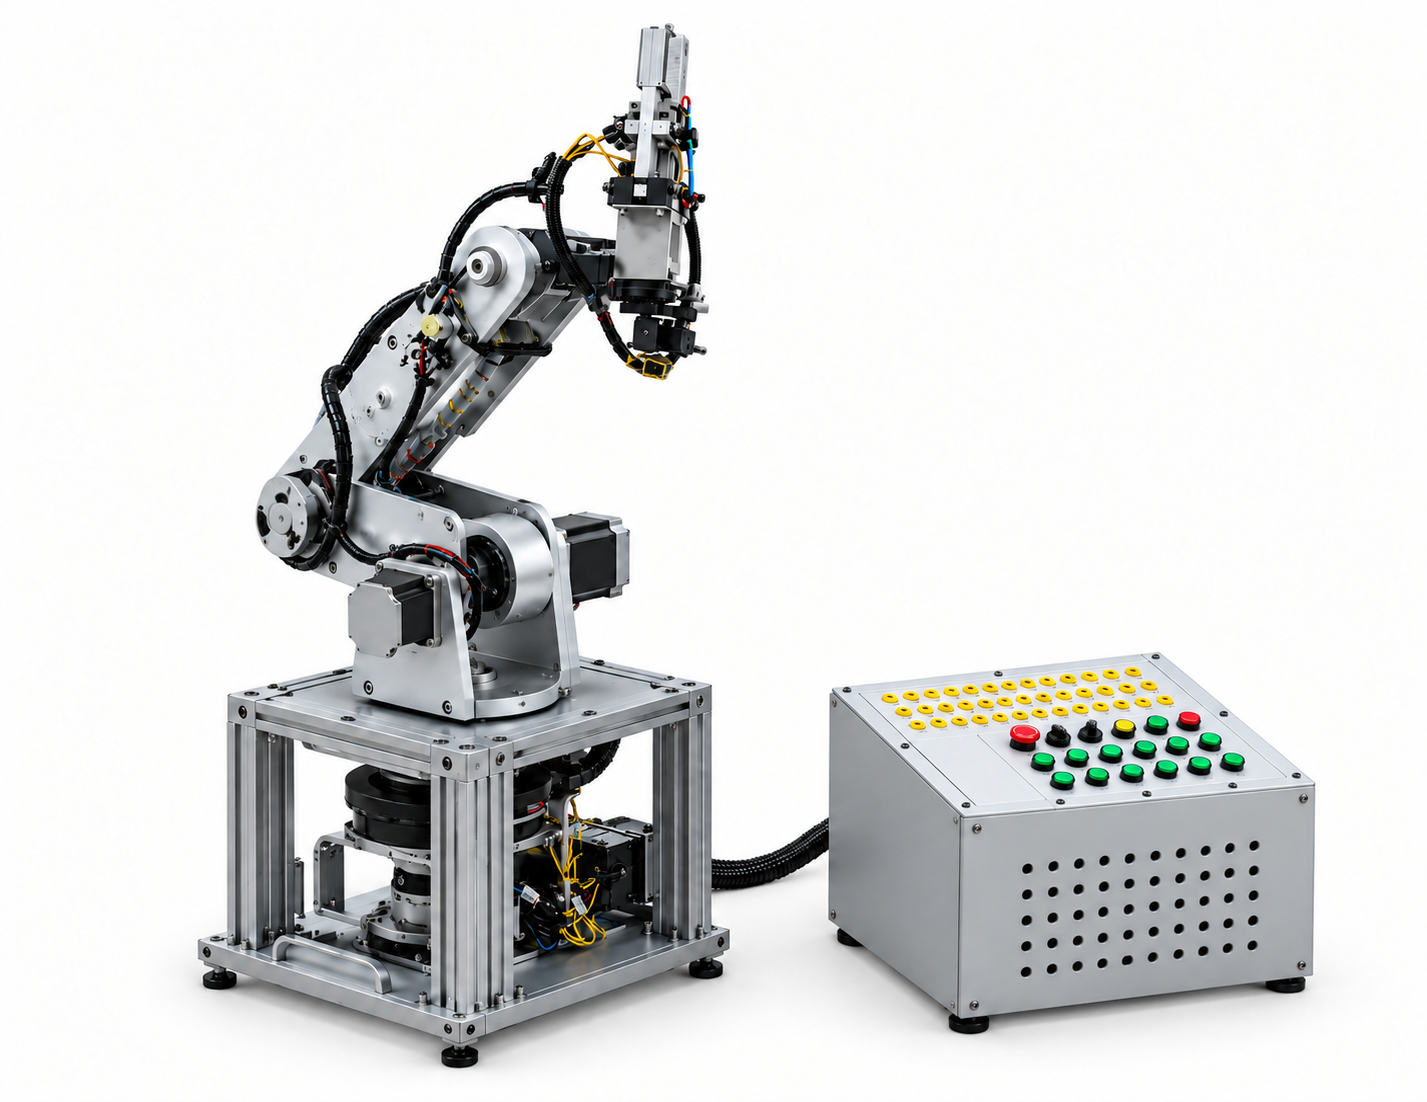
\includegraphics[width=10cm]{brazo.png}%
				}%
			}%
		}
		\centering
		
		% Encabezado institucional
		{\fontsize{18}{24}\selectfont 
			UNIVERSIDAD MAYOR DE SAN ANDRÉS \\
			FACULTAD DE INGENIERÍA \\
			CARRERA DE INGENIERÍA ELECTRÓNICA \par}
		
		\vspace{0.5cm}
		
		% Logo 
		
\includegraphics[width=0.25\textwidth]{Umsa-logo.svg.png}
		
		% Título del informe
		\rule{\textwidth}{0.5pt} % Línea decorativa
		{\Huge\bfseries \\ INFORME DE LABORATORIO 2 \par}
		\rule{\textwidth}{0.5pt} % Línea decorativa
		{\Large\bfseries \\ETN-902, ETN-1000, ETN-1034\par}
		
		
		% Sección de integrantes
		\begin{flushleft}
			{\Large\bfseries ESTUDIANTES: \par}
			\vspace{0.2cm}
			{\large
				\begin{tabular}{l}
					UNIV. CALLATA BAUTISTA DANIELA JHANIN\\
					UNIV. CARI ULURI CRISTHIAN DANIEL\\
					UNIV. GUTIERREZ PONCE CHRISTIAN YAMIL\\
					UNIV. MORALES CORICO NATALIA KATERINA\\
					UNIV. NINA FERNANDEZ DIEGO JOSUE\\
					UNIV. VILLCA YARARI GIOVANNI ALEXANDER
				\end{tabular} \par}
			\vspace{0.4cm}
			
			
			% Sección de docente
			{\Large\bfseries DOCENTE: \par}
			\vspace{0.2cm}
			{\large
				\begin{tabular}{l}
					ING. JORGE ANTONIO NAVA AMADOR
				\end{tabular} \par}
			
			\vspace{0.4cm}
			
			% Sección de auxiliares
			{\Large\bfseries AUXILIARES: \par}
			\vspace{0.2cm}
			{\large
				\begin{tabular}{l}
					UNIV. FABIAN MANUEL PLATA VARGAS\\
					UNIV. LIMBER AJNOTA CAHUAYA\\
					UNIV. FRANZ CHOQUE
				\end{tabular} \par}
		\end{flushleft}
		
		% Pie de página
		{\large 
			La Paz - Bolivia }
	\end{titlepage}
	\newpage
	
	\tableofcontents
	\newpage
	
\section{Levantamiento P\&ID según ANSI/ISA-S5.1-2009}
\label{sec:pid_brazo}

\begin{instrucciones}
	\textbf{Objetivo del bloque.} Generar la Versión~2.0 del plano P\&ID del brazo robótico XK~ls5b, aplicando el estándar ANSI/ISA-S5.1-2009 y corrigiendo las discrepancias detectadas en el Laboratorio~1.
	
	\textbf{Pasos mínimos requeridos:}
	\begin{enumerate}[leftmargin=*]
		\item Inventariar todos los instrumentos, actuadores y controladores del brazo, articulación por articulación (5~rotacionales + pinza).
		\item Asignar el código de letras ISA (variable medida + función), respetando la extensión al dominio de \emph{motion control} indicada en la Tabla~\ref{tab:letras_isa}.
		\item Dibujar el P\&ID en AutoCAD Electrical: líneas de proceso mecánico $=1{,}0$~mm; líneas de señal electrónica $=0{,}25$~mm; ver Tabla~\ref{tab:calibres}.
		\item Diferenciar gráficamente señales digitales (STEP/DIR, límites) y señales analógicas mediante los estilos ISA~5.1 §5.5.
		\item Ubicar el símbolo de cada instrumento (círculo con/sin línea horizontal o hexágono) según su localización funcional (campo, panel, PLC/PIC).
		\item Incluir el cajetín formal de la Carrera de Ingeniería Electrónica y marcar la revisión como \emph{Versión~2.0}.
	\end{enumerate}
	
	\textbf{Responsable:} \rule{6cm}{0.4pt}
\end{instrucciones}

% -----------------------------------------------------------------
\subsection{Adaptación de la norma ISA-5.1 a un manipulador robótico}
\label{subsec:isa_adaptacion}

La norma ANSI/ISA-S5.1-2009 fue concebida para procesos continuos con flujos másicos (líquidos, gases, sólidos a granel), donde las variables típicas son nivel, temperatura, presión y caudal. El brazo XK~ls5b es, en cambio, un \textbf{sistema discreto de manipulación cinemática} cuya variable física dominante es la \emph{posición angular} $q_i(t)$ de cada articulación. La aplicación de la norma exige entonces reinterpretar el código de la primera letra hacia variables mecánicas de movimiento, sin alterar el significado de las letras sucesivas de función.

La Tabla~\ref{tab:letras_isa} resume las equivalencias adoptadas para este trabajo.

\begin{table}[H]
	\centering\small
	\caption{Reasignación del código de letras ISA-5.1 al dominio del brazo XK~ls5b.}
	\label{tab:letras_isa}
	\begin{tabular}{@{}c l p{6.2cm}@{}}
		\toprule
		\textbf{Letra} & \textbf{Definición ISA} & \textbf{Aplicación al brazo} \\
		\midrule
		Z & Posición o dimensión mecánica & Ángulo articular $q_i$; detección de posición de referencia (\emph{home}) por efecto Hall \\
		S & Velocidad o frecuencia         & Frecuencia STEP entregada al driver bipolar (Hz) \\
		Y & Evento, estado o presencia    & Fin de carrera de la pinza; señales lógicas discretas \\
		H & Manual (\emph{Hand})          & Botones de paro de emergencia y comando manual \\
		I & Corriente eléctrica           & Corriente de fase del motor stepper (indicador de bloqueo/carga) \\
		\midrule
		E & \multicolumn{2}{l}{Función sucesiva: elemento primario (sensor).} \\
		T & \multicolumn{2}{l}{Función sucesiva: transmisor.} \\
		S & \multicolumn{2}{l}{Función sucesiva: switch (interruptor).} \\
		C & \multicolumn{2}{l}{Función sucesiva: control.} \\
		I & \multicolumn{2}{l}{Función sucesiva: indicación.} \\
		Y & \multicolumn{2}{l}{Función sucesiva: cómputo, conversión o relé.} \\
		\bottomrule
	\end{tabular}
\end{table}

\textbf{Consecuencia práctica.} El driver bipolar situado entre el PIC y la bobina del motor se codifica como \texttt{SY} (\emph{conversor de comando de velocidad hacia potencia de fases}), y no como una válvula ni como un controlador independiente: la lógica de control reside íntegramente en el PIC. De igual modo, los sensores Hall no se rotulan como transmisores continuos (\texttt{ZT}), sino como \emph{switches} de posición de referencia (\texttt{ZSH}), pues su función en el hardware existente es exclusivamente de \emph{homing} y no de realimentación continua (véase §5 del informe del Laboratorio~1).

% -----------------------------------------------------------------
\subsection{Convenciones de calibres de línea}
\label{subsec:calibres}

La Guía del Laboratorio~N.\textsuperscript{o}~2 fija dos calibres normativos (0{,}25~mm para señal y 1{,}0~mm para proceso). Para preservar la legibilidad del plano en formato A3 y facilitar la impresión del anexo, se extiende esta convención al conjunto completo de trazos del brazo:

\begin{table}[H]
	\centering\small
	\caption{Calibres y estilos de línea empleados en el P\&ID V2.0.}
	\label{tab:calibres}
	\begin{tabular}{@{}l c l@{}}
		\toprule
		\textbf{Trazo} & \textbf{Grosor (mm)} & \textbf{Estilo (ISA-5.1 §5.5)} \\
		\midrule
		Cuerpo mecánico (eslabón, reductor, acople) & 1{,}0 & Continuo sólido \\
		Alimentación de potencia AC/DC              & 0{,}50 & Continuo, etiqueta de tensión \\
		Señal digital (STEP, DIR, ENABLE)           & 0{,}25 & Continuo con doble barra oblicua \\
		Señal discreta on/off (final de carrera)    & 0{,}25 & Guiones cortos \\
		Señal analógica (Hall acondicionada, $I_\text{fase}$) & 0{,}25 & Guiones largos \\
		Función lógica interna del PIC              & 0{,}25 & Guión–punto–guión \\
		\bottomrule
	\end{tabular}
\end{table}

% -----------------------------------------------------------------
\subsection{Inventario ISA por articulación}
\label{subsec:inventario}

El brazo XK~ls5b posee \textbf{seis grados de libertad}: cinco articulaciones rotacionales $q_1\ldots q_5$ (base, hombro, codo, giro de muñeca, inclinación de muñeca) y una pinza $q_6$. Cada articulación se agrupa como un \emph{lazo funcional} independiente numerado 101–106, tal como exige el Punto~2 de la sección 3.1 de la Guía. La estructura repetitiva por articulación se refleja en el patrón de instrumentación de la Tabla~\ref{tab:inventario}.

\begin{longtable}{@{}c l p{5.4cm} l c@{}}
	\caption{Inventario ISA-5.1 de la instrumentación del brazo XK~ls5b.}
	\label{tab:inventario}\\
	\toprule
	\textbf{Lazo} & \textbf{Tag} & \textbf{Descripción funcional} & \textbf{Hardware} & \textbf{Ubic.} \\
	\midrule
	\endfirsthead
	\multicolumn{5}{c}{\tablename\ \thetable\ (continuación)}\\
	\toprule
	\textbf{Lazo} & \textbf{Tag} & \textbf{Descripción funcional} & \textbf{Hardware} & \textbf{Ubic.} \\
	\midrule
	\endhead
	\bottomrule
	\endfoot
	% -------- Lazo 101 -- Base (q1) --------
	101 & ZSH-101 & Switch Hall de posición de referencia (homing) & Sensor Hall base   & C \\
	101 & IY-101  & Aislamiento galvánico PIC$\rightarrow$driver     & Optoacoplador       & C \\
	101 & SY-101  & Conversor de comando STEP/DIR a fases            & Driver bipolar NEMA & C \\
	101 & SIC-101 & Control de perfil de velocidad de paso           & Función lógica PIC  & P \\
	\midrule
	% -------- Lazo 102 -- Hombro (q2) --------
	102 & ZSH-102 & Switch Hall de posición de referencia (homing) & Sensor Hall hombro & C \\
	102 & IY-102  & Aislamiento galvánico PIC$\rightarrow$driver     & Optoacoplador       & C \\
	102 & SY-102  & Conversor de comando STEP/DIR a fases            & Driver bipolar NEMA & C \\
	102 & SIC-102 & Control de perfil de velocidad de paso           & Función lógica PIC  & P \\
	\midrule
	% -------- Lazo 103 -- Codo (q3) --------
	103 & ZSH-103 & Switch Hall de posición de referencia (homing) & Sensor Hall codo    & C \\
	103 & IY-103  & Aislamiento galvánico PIC$\rightarrow$driver     & Optoacoplador       & C \\
	103 & SY-103  & Conversor de comando STEP/DIR a fases            & Driver bipolar NEMA & C \\
	103 & SIC-103 & Control de perfil de velocidad de paso           & Función lógica PIC  & P \\
	\midrule
	% -------- Lazo 104 -- Giro de muñeca (q4) --------
	104 & ZSH-104 & Switch Hall de posición de referencia (homing) & Sensor Hall $q_4$   & C \\
	104 & IY-104  & Aislamiento galvánico PIC$\rightarrow$driver     & Optoacoplador       & C \\
	104 & SY-104  & Conversor de comando STEP/DIR a fases            & Driver bipolar NEMA & C \\
	104 & SIC-104 & Control de perfil de velocidad de paso           & Función lógica PIC  & P \\
	\midrule
	% -------- Lazo 105 -- Inclinación de muñeca (q5) --------
	105 & ZSH-105 & Switch Hall de posición de referencia (homing) & Sensor Hall $q_5$   & C \\
	105 & IY-105  & Aislamiento galvánico PIC$\rightarrow$driver     & Optoacoplador       & C \\
	105 & SY-105  & Conversor de comando STEP/DIR a fases            & Driver bipolar NEMA & C \\
	105 & SIC-105 & Control de perfil de velocidad de paso           & Función lógica PIC  & P \\
	\midrule
	% -------- Lazo 106 -- Pinza (q6) --------
	106 & ZSH-106 & Fin de carrera: pinza totalmente abierta       & Micro-switch        & C \\
	106 & ZSL-106 & Fin de carrera: pinza totalmente cerrada       & Micro-switch        & C \\
	106 & IY-106  & Aislamiento galvánico PIC$\rightarrow$driver     & Optoacoplador       & C \\
	106 & SY-106  & Conversor de comando a driver de pinza           & Driver bipolar      & C \\
	106 & YIC-106 & Controlador lógico de estado abrir/cerrar        & Función lógica PIC  & P \\
	\midrule
	% -------- Servicios compartidos --------
	--- & JC-001  & Controlador maestro de movimiento (kinemática)   & PIC principal       & P \\
	--- & HS-001  & Paro de emergencia enclavado                     & Botón hongo         & C \\
	--- & HS-002  & Habilitación manual (\emph{deadman})             & Pulsador            & C \\
\end{longtable}

\noindent\textbf{Clave de ubicación funcional:} \texttt{C}~=~montado en campo (círculo simple, sin línea); \texttt{P}~=~función compartida en el PIC (círculo con hexágono inscrito), según ISA-5.1 §5.4.

% -----------------------------------------------------------------
\subsection{Anticipación de la agrupación de lazos (Punto 2)}
\label{subsec:preview_lazos}

El inventario de la Tabla~\ref{tab:inventario} anticipa la agrupación exigida por el Punto~2 de la Sección 3.1: seis lazos funcionales, uno por articulación, más un bloque de servicios compartidos. Los lazos 101–105 son \emph{idénticos en topología} (\texttt{ZSH}~+~\texttt{IY}~+~\texttt{SY}~+~\texttt{SIC}), lo que permitirá el uso de bloques de símbolos reutilizables en AutoCAD Electrical y una única leyenda tipográfica en el plano final. El lazo 106 se aparta ligeramente por incluir dos switches de fin de carrera y un controlador de estado lógico (\texttt{YIC}) en lugar de perfil de velocidad.


\section{Planos segun las normativa ISA5.1 y 60617/IEEE}

\subsection{Planos Electricos segun la NORMATIVA 60617}

\begin{figure}[H]
	\centering
	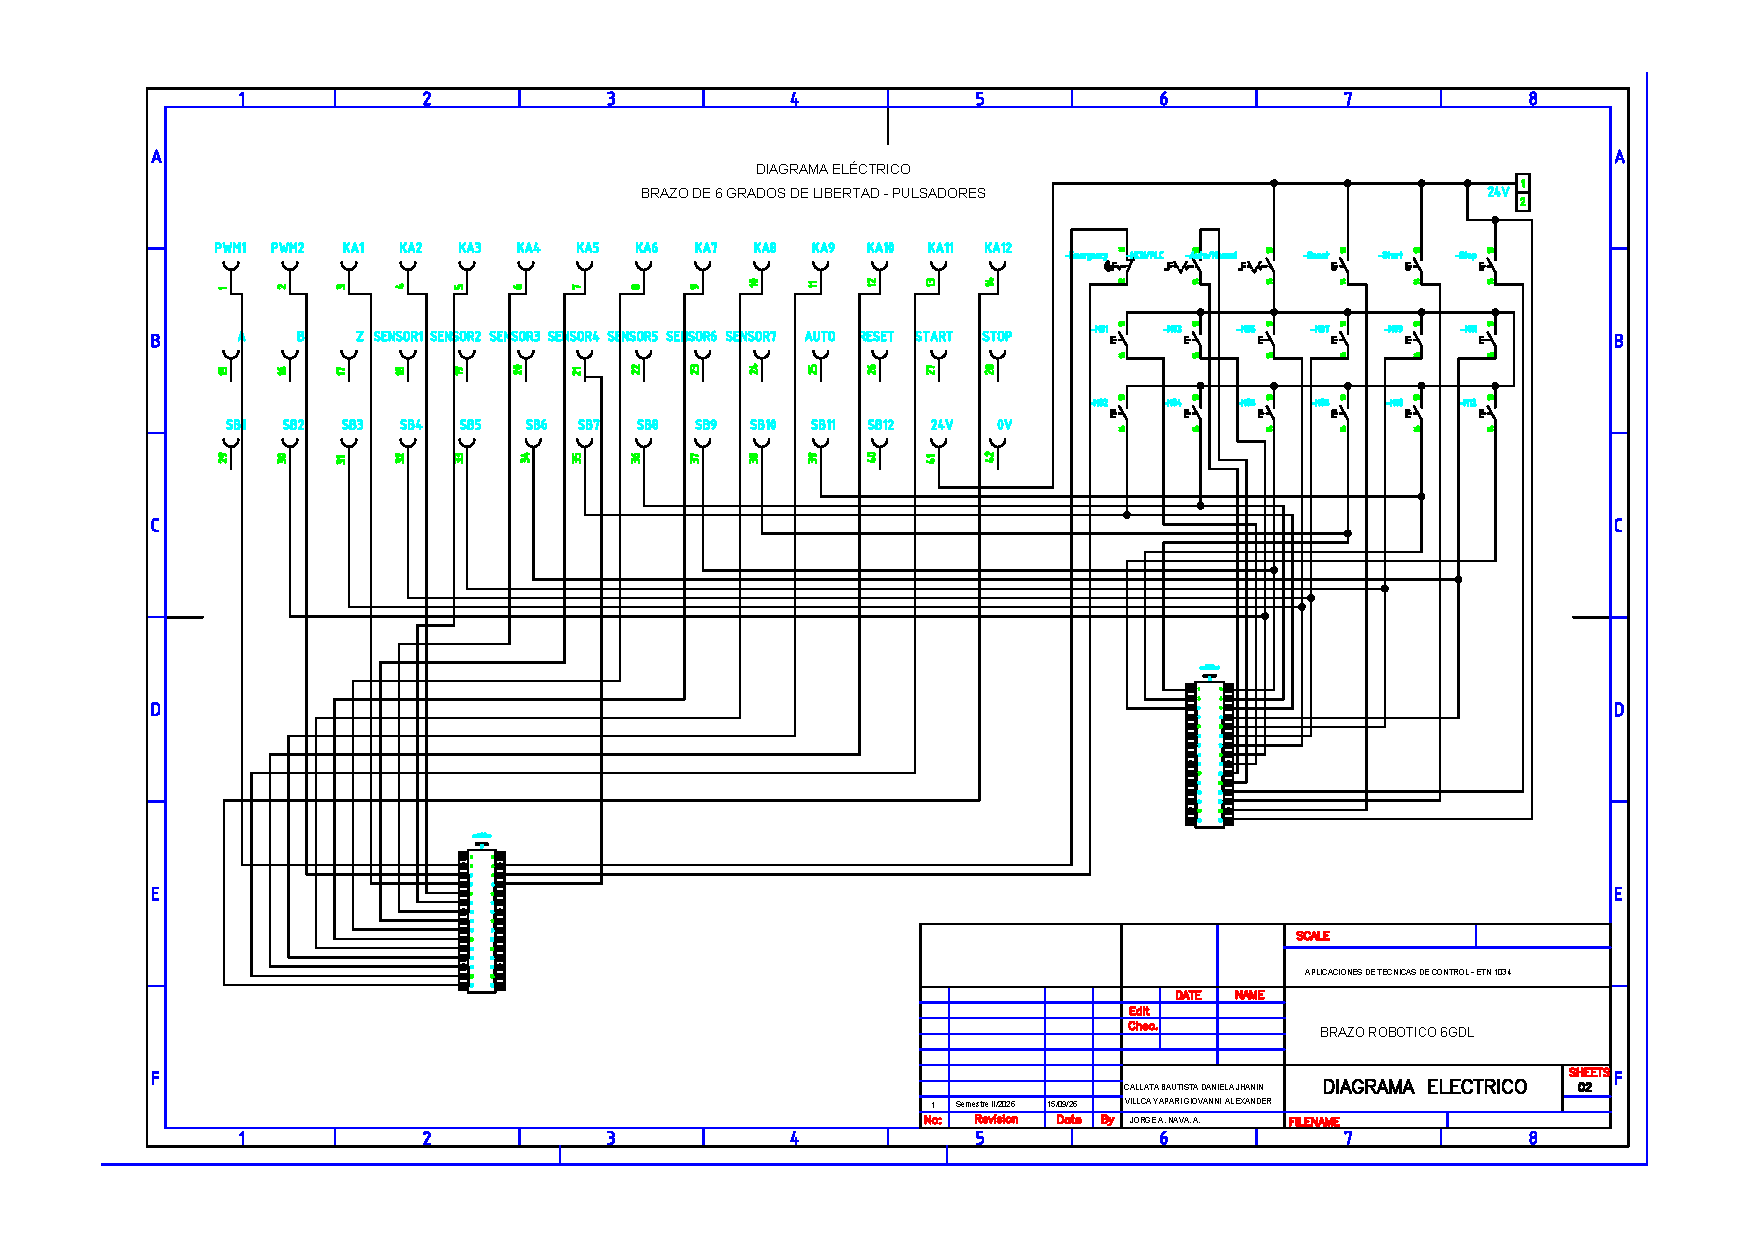
\includegraphics[width=\textwidth,height=0.78\textheight,keepaspectratio]{PULSADORES-Modelo.pdf}
	\caption{Diagrama eléctrico de pulsadores del brazo robótico de seis grados de libertad.}
	\label{fig:pulsadores_modelo}
\end{figure}


El análisis se restringe deliberadamente al
marco normativo eléctrico (\textbf{IEC 60617} para simbología,
\textbf{IEC 81346-2} para designación de referencias, y la
\textbf{normativa boliviana} vigente); el estándar de instrumentación
ANSI/ISA-S5.1-2009 será tratado en un documento separado, junto con los
diagramas P\&ID del sistema.

% =========================================================================
\subsubsection{Norma IEC 60617 — Símbolos gráficos para esquemas}
% =========================================================================

La \textbf{IEC 60617} —\emph{Graphical symbols for diagrams}— es la norma
internacional que define la simbología de los esquemas eléctricos y
electrónicos. Constituye el estándar de referencia mundial y está
adoptada en Europa como \textbf{EN 60617} y en España como
\textbf{UNE-EN 60617} (traducción oficial al español).

\subsubsection{Estructura de la norma y evolución}
En su edición impresa (1996–1999), IEC 60617 se organizó como una serie
de \textbf{trece partes numeradas}, cada una dedicada a un dominio
temático:

\begin{center}
	\small
	\begin{tabularx}{\linewidth}{@{}l X@{}}
		\toprule
		\textbf{Parte} & \textbf{Contenido} \\
		\midrule
		IEC 60617-1  & Introducción general (retirada e integrada en las siguientes partes).\\
		IEC 60617-2  & Elementos de símbolos, símbolos distintivos y otros símbolos de aplicación general.\\
		IEC 60617-3  & Conductores y dispositivos de conexión.\\
		IEC 60617-4  & Componentes pasivos básicos.\\
		IEC 60617-5  & Semiconductores y tubos electrónicos.\\
		IEC 60617-6  & Producción, transformación y conversión de la energía eléctrica.\\
		\textbf{IEC 60617-7}  & \textbf{Aparamenta y dispositivos de control y protección} (contactores, relés, pulsadores, selectores).\\
		IEC 60617-8  & Instrumentos de medida, lámparas y dispositivos de señalización.\\
		IEC 60617-9  & Telecomunicaciones — conmutación y equipos periféricos.\\
		IEC 60617-10 & Telecomunicaciones — transmisión.\\
		IEC 60617-11 & Esquemas y planos de instalación, arquitectónicos y topográficos.\\
		IEC 60617-12 & Operadores lógicos binarios.\\
		IEC 60617-13 & Operadores analógicos.\\
		\bottomrule
	\end{tabularx}
\end{center}

\begin{norma}
	Desde 2012 la IEC dejó de publicar las partes 2 a 13 por separado y las
	consolidó en una \textbf{base de datos en línea} (IEC 60617 DB), que
	contiene alrededor de 1\,900 símbolos y constituye la fuente oficial
	actual del estándar. Las partes numeradas siguen citándose porque la
	literatura académica y las herramientas CAD conservan la referencia
	original.
\end{norma}

\subsubsection{Partes de IEC 60617 aplicables al tablero de pulsadores}
De las trece partes, tres son directamente aplicables a este trabajo:

\begin{itemize}[leftmargin=1.4em]
	\item \textbf{IEC 60617-2} — provee la simbología de los elementos
	auxiliares del plano: marcos de agrupación, líneas de conexión,
	puntos de unión, indicadores de tierra, y las convenciones para
	\emph{cross-references} entre hojas.
	\item \textbf{IEC 60617-3} — cubre la representación de los
	\emph{conductores} (una línea, bus, mazo) y de los
	\emph{dispositivos de conexión}: bornes, regletas de bornes y
	conectores multivía. En este plano rige los conectores
	\texttt{-X1} y \texttt{-X2} de interconexión al controlador.
	\item \textbf{IEC 60617-7} — es la parte \textbf{principal} para este
	tablero: define los símbolos de contactos normalmente abiertos
	(NA) y normalmente cerrados (NC) de pulsadores, la retención
	mecánica de la seta de emergencia, los selectores de dos
	posiciones (\texttt{MCU/PLC}, \texttt{Auto/Manual}) y los
	contactos auxiliares de relé (\texttt{KA1\dots KA12}).
\end{itemize}

\begin{insertar}
	\textbf{Símbolos investigados por el autor.} Insertar aquí la tabla de
	símbolos utilizados en el plano con su código IEC 60617 correspondiente
	(NA, NC, seta de emergencia con retención, selector, contacto auxiliar,
	bornera). Los enlaces recopilados por el autor van en esta sección.
\end{insertar}

% =========================================================================
\subsubsection{Normativa boliviana aplicable}
% =========================================================================

En Bolivia el organismo rector de la normalización técnica es el
\textbf{Instituto Boliviano de Normalización y Calidad (IBNORCA)}. Las
normas eléctricas bolivianas se identifican con el prefijo \textbf{NB}
seguido de un número, y son elaboradas por el Comité Técnico de
Normalización 14.8 \emph{Instalaciones eléctricas}, con participación
de la Facultad de Ingeniería — UMSA, el Colegio de Ingenieros
Electricistas y Electrónicos (CIEE), la Sociedad de Ingenieros de
Bolivia (SIB) y las distribuidoras eléctricas nacionales.

\subsubsection{NB 777 — Instalaciones eléctricas interiores en baja tensión}
La norma boliviana rectora en el ámbito eléctrico es la
\textbf{NB 777:2024} —\emph{Diseño y construcción de instalaciones
	eléctricas interiores en baja tensión}—, presentada oficialmente por
IBNORCA en febrero de 2025. Está estructurada en varias partes
(NB 777-1: definiciones y principios; NB 777-3: instalaciones
específicas y hospitales; NB 777-4: materiales) y aplica a
circuitos con tensión nominal máxima de 1\,000\,V CA o 1\,500\,V CC.

\begin{observa}
	NB 777 está pensada principalmente para \textbf{instalaciones
		eléctricas de edificios} (residenciales, comerciales, industriales,
	hospitalarios), no para el equipamiento eléctrico interno de máquinas.
	Su alcance directo sobre el tablero de pulsadores del brazo se limita
	a: (a) la acometida de alimentación al tablero, (b) el sistema de
	puesta a tierra, (c) las protecciones aguas arriba, y (d) el color de
	los conductores del cableado externo. La simbología detallada del
	tablero de mando se rige por IEC 60617 e IEC 60204-1.
\end{observa}

\subsubsection{IEC 60204-1 — Equipo eléctrico de las máquinas}
Para el tablero de mando de la máquina —el brazo robótico— la norma
técnicamente aplicable es \textbf{IEC 60204-1:2016} (con Amd.\ 1:2021)
—\emph{Safety of machinery — Electrical equipment of machines. Part 1:
	General requirements}—. Aunque no ha sido emitida como norma boliviana
explícita, es de \textbf{adopción de facto} en la industria y la
academia bolivianas, y regula tres aspectos que aparecen directamente
en el plano:

\begin{itemize}[leftmargin=1.4em]
	\item \textbf{Cadena de paro de emergencia} (cláusula 9.2.5.4):
	contacto normalmente cerrado, con retención mecánica, cableado
	de forma directa (\emph{hardwired}) en la línea de mando. La
	seta \texttt{Emergency} del plano cumple esta disposición.
	\item \textbf{Código de colores de pulsadores} (cláusula 10.2):
	rojo para paro/emergencia, verde para marcha, amarillo para
	anormalidad, azul para acción obligatoria, blanco/gris/negro
	para funciones generales.
	\item \textbf{Código de colores de luces piloto} (cláusula 10.3):
	rojo emergencia, amarillo anormalidad, verde condición normal,
	azul acción obligatoria, blanco confirmación.
\end{itemize}

\begin{center}
	\small
	\begin{tabularx}{\linewidth}{@{}l l X@{}}
		\toprule
		\textbf{Color} & \textbf{Pulsador (IEC 60204-1)} & \textbf{Aplicación en este tablero} \\
		\midrule
		Rojo     & Paro / Emergencia          & \texttt{STOP}, \texttt{Emergency}.\\
		Verde    & Marcha / Arranque          & \texttt{START}.\\
		Amarillo & Reset / Retorno            & \texttt{RESET}.\\
		Blanco   & Función general (jog)      & \texttt{SB1\dots SB12} (movimiento manual de ejes).\\
		Azul     & Acción obligatoria         & \texttt{AUTO} (cambio a modo automático).\\
		\bottomrule
	\end{tabularx}
\end{center}

% =========================================================================
\subsubsection{Designación de referencias — IEC 81346-2}
% =========================================================================

La \textbf{IEC 81346-2:2019} (antes IEC 61346-2) establece la
\emph{nomenclatura de identificación de componentes} de un sistema
eléctrico mediante una \textbf{letra de clase} precedida por el signo
\texttt{-}. Es la norma que respalda el uso de las letras \texttt{K,
	M, S, X} que aparecen en el plano.

\begin{center}
	\small
	\begin{tabularx}{\linewidth}{@{}c l X@{}}
		\toprule
		\textbf{Letra} & \textbf{Clase de objeto} & \textbf{Ejemplos en este tablero} \\
		\midrule
		\texttt{K} & Relés, contactores, dispositivos de conmutación de mando & \texttt{-KA1\dots-KA12} (relés auxiliares).\\
		\texttt{M} & Motores y actuadores eléctricos                          & Motores de los 6 ejes del brazo (en la hoja de potencia).\\
		\texttt{S} & Dispositivos de mando manual y sensores de posición      & \texttt{-SB1\dots-SB12} (pulsadores), \texttt{-S0} (emergencia), \texttt{-S1, -S2} (selectores).\\
		\texttt{H} & Dispositivos de señalización                              & Luces piloto \texttt{-HL$n$} (no presentes en esta hoja).\\
		\texttt{X} & Terminales, bornes, conectores                            & \texttt{-X1, -X2} (conectores multipin al controlador).\\
		\texttt{Q} & Aparatos de conmutación de potencia                       & Interruptor general del tablero (hoja de potencia).\\
		\texttt{F} & Dispositivos de protección                                & Interruptores termomagnéticos, fusibles (hoja de potencia).\\
		\bottomrule
	\end{tabularx}
\end{center}

\subsection*{¿Está bien usar K, M, S, X en el plano?}

Sí, es la práctica \textbf{normativamente correcta} bajo IEC 81346-2 y
mejora la legibilidad del plano para el usuario: permite identificar
la función de un componente por su letra sin recurrir a la leyenda.
No obstante, la designación exige \textbf{consistencia} entre hojas
del mismo plano y entre planos del mismo proyecto:

\begin{observa}
	En la hoja actual se observa una \textbf{inconsistencia menor a
		resolver}: el bloque izquierdo emplea \texttt{KA1\dots KA12} para los
	contactos auxiliares de los relés, mientras que la cadena de mando de
	la derecha emplea \texttt{-M01\dots-M12} para lo que parecen ser los
	mismos contactos actuando sobre cada motor. Dado que la letra
	\texttt{M} bajo IEC 81346-2 se reserva a los \emph{motores}, se
	recomienda una de estas dos acciones:
	
	\begin{enumerate}[label=(\alph*),leftmargin=1.6em]
		\item \textbf{Renombrar} los contactos de la derecha como
		\texttt{-K01\dots-K12} (o \texttt{-KA13\dots-KA24} si son relés
		auxiliares distintos de los del lado izquierdo), lo que
		alineará la designación con la norma.
		\item \textbf{Mantener} la designación actual, agregando en la
		\emph{leyenda del plano} la declaración explícita:
		\emph{``$-$M$n$: contacto auxiliar asociado al motor $n$
			del brazo''}.
	\end{enumerate}
\end{observa}

% =========================================================================
\subsubsection*{Modificaciones sugeridas para el contexto boliviano}
% =========================================================================

Considerando el marco normativo boliviano y la práctica local, se
recomiendan las siguientes modificaciones sobre el plano actual para
facilitar su lectura y su aceptación en revisiones técnicas nacionales
(revisiones del Ing.\ docente, publicación en repositorios, o
integración a un informe evaluado por CIEE):

\begin{enumerate}[leftmargin=1.4em]
	\item \textbf{Rotular en español los pulsadores de la cadena de
		mando.} Actualmente aparecen \texttt{Emergency}, \texttt{Reset},
	\texttt{Start}, \texttt{Stop}. Reemplazar por
	\texttt{Emergencia}, \texttt{Reposición}, \texttt{Marcha},
	\texttt{Paro} —consistente con el resto del plano y con la
	práctica IBNORCA de documentación técnica en español.
	
	\item \textbf{Incorporar el código de colores IEC 60204-1} en las
	etiquetas del plano (aunque el plano sea monocromo, indicar
	junto a cada pulsador el color de la cabeza física:
	\texttt{Paro (rojo)}, \texttt{Marcha (verde)},
	\texttt{Reposición (amarillo)}, \texttt{Emergencia (rojo
		seta)}).
	
	\item \textbf{Añadir luces piloto} \texttt{-HL1\dots-HL$n$} para
	confirmación visual del estado del tablero: presencia de 24\,V,
	modo automático/manual, marcha, paro y falla. Su omisión es
	una desviación menor respecto a la cláusula 10.3 de IEC
	60204-1.
	
	
	\subsubsection{Link Para viasulizar la simbologia de la normativa 60617\IEEE}
	
	\begin{figure}[H]
		\centering
		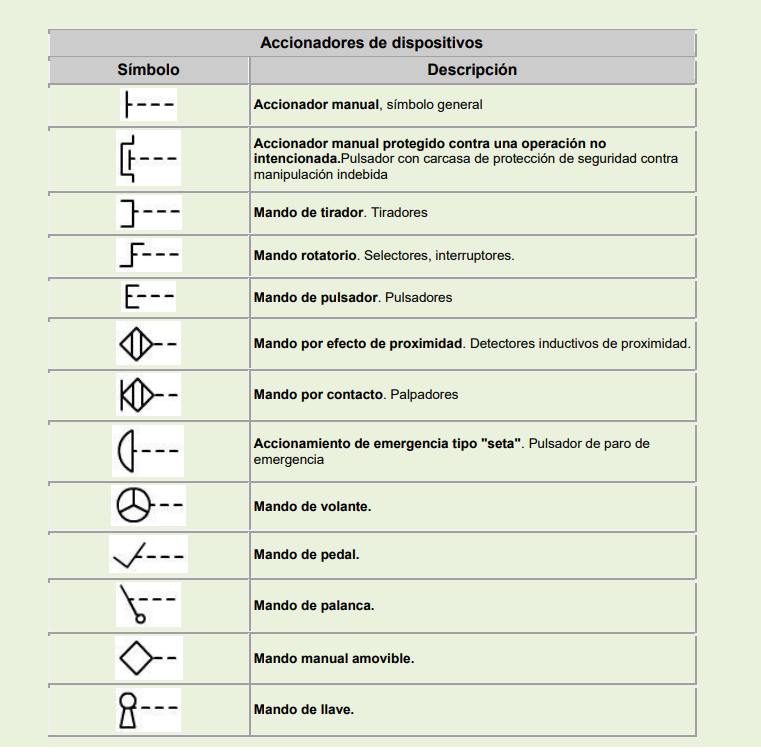
\includegraphics[width=\linewidth,height=0.70\textheight,keepaspectratio]{Normativa60617.png}
		\caption{Ejemplo de simbologia Electrica Normativa ISA5.1}
		\label{fig:normativa60617}
	\end{figure}
	
	
	
	\url{https://alfredoch66.wordpress.com/wp-content/uploads/2012/12/simbolos-electricos.pdf}
	
	
	
	
	% -----------------------------------------------------------------
	\section{Discrepancias corregidas respecto al Laboratorio 1 (Kaizen)}
	\label{subsec:kaizen}
	
	En cumplimiento del objetivo de \emph{Estratificación de Versiones} (§1.1 de la Guía), la Versión~2.0 del P\&ID incorpora las siguientes correcciones respecto al plano original:
	
	\begin{enumerate}[leftmargin=*]
		\item \textbf{Reclasificación del driver bipolar} como conversor \texttt{SY} (no como controlador \texttt{SC} o \texttt{JC}). La lógica de control reside en el PIC; el driver sólo traduce la secuencia STEP/DIR en energización de fases.
		\item \textbf{Reclasificación de los sensores Hall} como switches de posición de referencia (\texttt{ZSH}) y no como transmisores continuos (\texttt{ZT}), reflejando fielmente que el brazo opera en lazo abierto en posición.
		\item \textbf{Explicitación de los optoacopladores} \texttt{IY-1xx} como elementos normados de aislamiento galvánico, previamente representados como interconexiones informales.
		\item \textbf{Numeración secuencial por articulación} (101–106), en reemplazo de la agrupación previa por tipo de instrumento.
		\item \textbf{Diferenciación gráfica} entre señales digitales STEP/DIR (\texttt{SY}) y señales discretas de fin de carrera (\texttt{ZSH}/\texttt{ZSL}) mediante los estilos de línea de la Tabla~\ref{tab:calibres}.
		\item \textbf{Incorporación normativa} de \texttt{HS-001} y \texttt{HS-002} como instrumentos manuales de seguridad, y no como anotaciones informales en el margen del plano.
		\item \textbf{Cajetín formal} de la Carrera de Ingeniería Electrónica con revisión, fecha, escala y nombre de la escuadra.
	\end{enumerate}
	
	\subsection{Limitación explícita del alcance del plano}
	\label{subsec:limitacion}
	
	El P\&ID V2.0 documenta el \emph{estado as-built} del brazo bajo su arquitectura actual (lazo abierto en posición, sensores en función de homing y seguridad). Los instrumentos adicionales requeridos para el cierre del lazo por realimentación de estados —encoders incrementales o absolutos por articulación, transmisores de par— son objeto de las materias ETN-1034 y ETN-902 en el análisis de rediseño y se documentarán en una \emph{Versión 3.0} del plano una vez validada la propuesta de instrumentación en simulación.
	
	
	
	
	
	% BASE DE DATOS
	\newpage
	\section{Tareas de los estudiantes de Bases de Datos}
	\subsection{Diseño de maquetas y patrones de interfaz de usuario}
	Se presentan las maquetas esquemáticas de los dos entornos obligatorios: la interfaz humano-máquina (HMI) local de la planta y el panel de control web del sistema de planificación de recursos empresariales (ERP). Ambos se relacionan con las entidades identificadas en el modelo de datos de la Guía N.\textsuperscript{o}~1 (\campo{EJE}, \campo{LECTURA_TELEMETRIA}, \campo{ALERTA} y \campo{SESION_OPERACION}) y con las ampliaciones propuestas en la sección~\ref{sec:campos}.
	
	\subsubsection{Pantalla HMI de planta (PanelView táctil de 5,7 pulgadas)}
	
	La interfaz local simplificada está orientada al operador de campo. Muestra la posición estimada como variable de proceso ($PV$), la consigna o \textit{setpoint} ($SP$), el estado lógico de los actuadores y el estado de la parada de emergencia. La indicación en pantalla no sustituye al pulsador físico de emergencia ni a su circuito de seguridad.
	
	\begin{center}
		\scalebox{0.85}{%
			\begin{tikzpicture}[font=\small]
				\tikzset{every node/.append style={execute at begin node=\sffamily}}
				\draw[rounded corners=6pt, thick, fill=gray!5] (0,0) rectangle (12,8);
				
				% Header
				\draw[fill=gray!25] (0,7.2) rectangle (12,8);
				\node[font=\bfseries\footnotesize] at (6,7.6) {BRAZO XK-JS5B -- CONTROLADOR PIC 16F1946};
				
				% Eje tabs
				\foreach \eje/\posicion in {1/0.3,2/2.25,3/4.2,4/6.15,5/8.1,6/10.05}{
					\draw[rounded corners=2pt, fill=blue!12] (\posicion,6.5) rectangle ++(1.6,0.6);
					\node at (\posicion+0.8,6.8) {Eje \eje};
				}
				\node[anchor=west, font=\scriptsize] at (0.1,6.2) {Selector de eje activo (numero\_eje)};
				
				% PV display
				\draw[rounded corners=4pt, thick, fill=teal!10] (0.5,4) rectangle (5.5,6.0);
				\node[font=\bfseries] at (3,5.55) {PV -- Posición estimada};
				\node[font=\Large\bfseries] at (3,4.9) {$\theta \approx 42{,}5^{\circ}$};
				\node[font=\scriptsize] at (3,4.3) {(a partir de pasos y dirección)};
				
				% SP display
				\draw[rounded corners=4pt, thick, fill=orange!10] (6.5,4) rectangle (11.5,6.0);
				\node[font=\bfseries] at (9,5.55) {SP -- Consigna angular};
				\node[font=\Large\bfseries] at (9,4.9) {$\theta_{\mathrm{d}} = 90{,}0^{\circ}$};
				\node[font=\scriptsize] at (9,4.3) {(referencia ingresada por el operador)};
				
				% Status LEDs
				\draw[fill=green!20, draw=green!50!black] (1.2,3.1) circle (0.32);
				\node[font=\scriptsize] at (1.2,2.55) {MARCHA};
				\draw[fill=red!20, draw=red!60!black] (4.5,3.1) circle (0.32);
				\node[font=\scriptsize] at (4.5,2.55) {PARO};
				\draw[fill=yellow!30, draw=orange!70!black] (7.8,3.1) circle (0.32);
				\node[font=\scriptsize, align=center] at (7.8,2.4) {FIN DE\\CARRERA};
				\draw[fill=gray!20, draw=gray!60!black] (10.8,3.1) circle (0.32);
				\node[font=\scriptsize] at (10.8,2.55) {DRIVER EN};
				
				% Emergency button
				\draw[rounded corners=8pt, thick, fill=red!70, draw=red!80!black] (3,0.4) rectangle (9,1.9);
				\node[font=\bfseries\normalsize, text=white] at (6,1.35) {PARADA DE EMERGENCIA};
				\node[font=\scriptsize, text=white] at (6,0.8) {Indicador del estado del circuito físico};
			\end{tikzpicture}
		}
	\end{center}
	
	
	\begin{figure}[H]
		\centering
		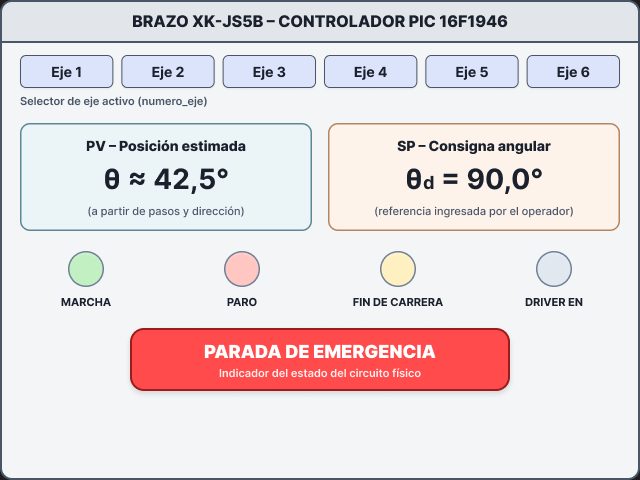
\includegraphics[width=0.6\textwidth]{hmi.png}
		\caption{Interfaz HMI diseñada en Figma.}
	\end{figure}
	
	\subsubsection{Panel de control del ERP web}
	
	La interfaz analítica está destinada a autoridades y personal científico. Incluye series temporales de posición estimada, una tabla de alarmas y un registro de auditoría de las acciones de los usuarios.
	
	\begin{center}
		\begin{tikzpicture}[font=\scriptsize]
			\tikzset{every node/.append style={execute at begin node=\sffamily}}
			\draw[rounded corners=4pt, thick, fill=gray!5] (0,0) rectangle (16,10);
			
			% Navbar
			\draw[fill=gray!25] (0,9) rectangle (16,10);
			\node[font=\bfseries\footnotesize] at (3.2,9.5) {ERP -- Brazo Robótico XK-JS5B};
			\foreach \etiqueta/\posicion in {Resumen/7.5,Histórico/9.7,Alarmas/12.0,Auditoría/14.2}{
				\node[font=\footnotesize] at (\posicion,9.5) {\etiqueta};
			}
			
			% Sidebar
			\draw[fill=blue!5] (0,0) rectangle (3,9);
			\node[font=\bfseries\footnotesize] at (1.5,8.6) {Filtros};
			\draw (0.3,7.7) rectangle (2.7,8.2); \node at (1.5,7.95) {Eje: [1--6]};
			\draw (0.3,6.7) rectangle (2.7,7.2); \node at (1.5,6.95) {Desde: [fecha]};
			\draw (0.3,5.7) rectangle (2.7,6.2); \node at (1.5,5.95) {Hasta: [fecha]};
			\draw[rounded corners=3pt, fill=blue!20] (0.3,4.6) rectangle (2.7,5.2); \node[font=\bfseries] at (1.5,4.9) {Aplicar};
			
			% Chart area
			\draw[thick] (3.3,5.3) rectangle (15.7,8.7);
			\node[font=\bfseries\footnotesize] at (9.5,8.4) {Histórico de posición angular estimada en función del tiempo};
			\draw[->] (3.7,5.6) -- (15.3,5.6);
			\draw[->] (3.7,5.6) -- (3.7,8.2);
			\node[anchor=west] at (3.85,8.0) {$\theta$ (grados)};
			\node[anchor=south east] at (15.2,5.65) {Tiempo};
			\draw[thick, blue] (3.9,5.9) -- (5.2,7.1) -- (6.5,6.4) -- (7.9,7.6) -- (9.3,6.9) -- (10.8,7.9) -- (12.2,6.6) -- (13.6,7.4) -- (15.0,6.8);
			
			% Alarm table
			\draw[thick] (3.3,2.6) rectangle (9.3,4.9);
			\node[font=\bfseries\footnotesize] at (6.3,4.65) {Tabla de alarmas};
			\draw (3.3,3.9) -- (9.3,3.9);
			\node[font=\bfseries\scriptsize] at (4.1,4.15) {Fecha};
			\node[font=\bfseries\scriptsize] at (5.4,4.15) {Eje};
			\node[font=\bfseries\scriptsize] at (6.7,4.15) {Tipo};
			\node[font=\bfseries\scriptsize] at (8.4,4.15) {Severidad};
			\foreach \altura in {3.5,3.1,2.7}{
				\draw[gray!40] (3.3,\altura) -- (9.3,\altura);
			}
			
			% Audit table
			\draw[thick] (9.6,2.6) rectangle (15.7,4.9);
			\node[font=\bfseries\footnotesize] at (12.65,4.65) {Auditoría de usuarios};
			\draw (9.6,3.9) -- (15.7,3.9);
			\node[font=\bfseries\scriptsize] at (10.6,4.15) {Usuario};
			\node[font=\bfseries\scriptsize] at (12.7,4.15) {Acción};
			\node[font=\bfseries\scriptsize] at (14.8,4.15) {Fecha};
			\foreach \altura in {3.5,3.1,2.7}{
				\draw[gray!40] (9.6,\altura) -- (15.7,\altura);
			}
		\end{tikzpicture}
	\end{center}
	
	\begin{figure}[H]
		\centering
		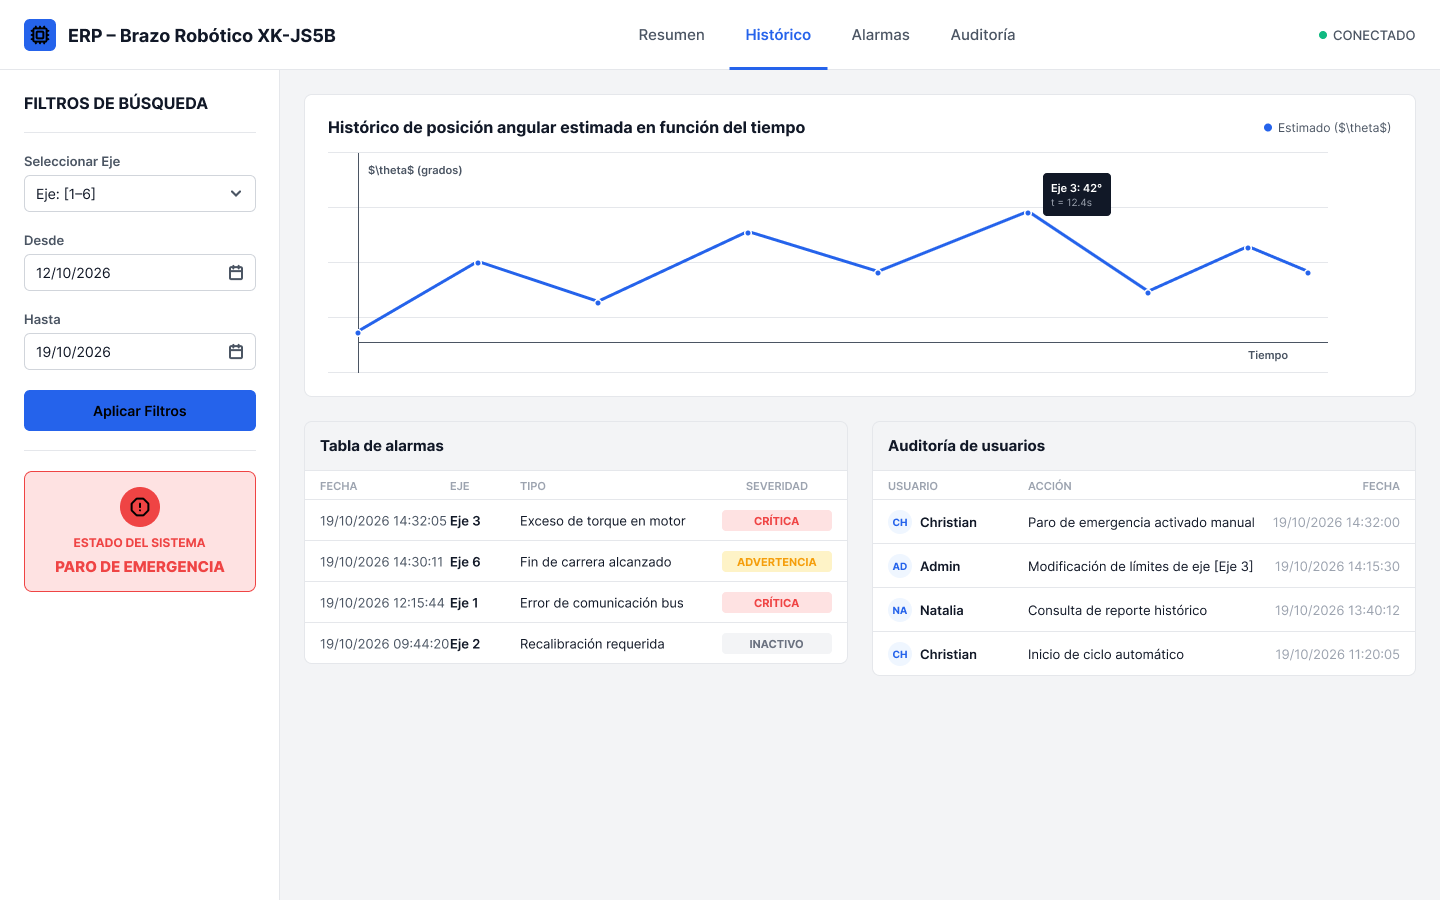
\includegraphics[width=1\textwidth]{dashboard.png}
		\caption{Panel de control web diseñado en Figma.}
	\end{figure}
	
	\subsubsection*{Paleta de colores y tipografía}
	\begin{itemize}[leftmargin=1.2em, itemsep=1pt]
		\item \textbf{Fondo neutro claro} (\texttt{gray!5}) para favorecer el contraste. La legibilidad debe comprobarse con la iluminación real de la planta.
		\item \textbf{Código de colores de estado}: verde (marcha/OK), rojo (paro/alarma crítica), ámbar (advertencia -- fin de carrera), gris (inactivo).
		\item \textbf{Tipografía sin serifas} en las maquetas, con valores $PV$ y $SP$ destacados, encabezados en negrita y etiquetas secundarias de menor tamaño, para facilitar la lectura del HMI.
		\item El indicador de parada de emergencia se distingue por su tamaño, su etiqueta y su fondo rojo saturado. Los colores mostrados son ilustrativos, no estados simultáneos de operación; las etiquetas complementan el color.
	\end{itemize}
	
	\subsection{Organigrama de vistas}
	
	El siguiente organigrama muestra la jerarquía de navegación propuesta entre las pantallas diseñadas.
	
	\begin{center}
		\begin{tikzpicture}[
			nodo/.style={rectangle, draw, rounded corners=3pt, fill=blue!8, minimum width=3.4cm, minimum height=0.9cm, align=center, font=\sffamily\small},
			hoja/.style={rectangle, draw, rounded corners=3pt, fill=violet!8, text width=2.5cm, minimum height=0.9cm, align=center, font=\sffamily\footnotesize},
			rel/.style={-{Latex[length=2mm]}, thick}
			]
			\node[nodo] (login) at (0,8) {Inicio de sesión};
			\node[nodo] (menu) at (0,6.3) {Menú principal};
			\node[nodo] (hmi) at (-5.8,4.3) {HMI local\\(PanelView)};
			\node[nodo] (dash) at (1.45,4.3) {Panel de control web};
			
			\node[hoja] (ejes) at (-5.8,2.3) {Selector de eje\\(1--6)};
			
			\node[hoja] (resumen) at (-2.9,2.3) {Resumen general};
			\node[hoja] (historico) at (0,2.3) {Histórico por eje};
			\node[hoja] (alarmas) at (2.9,2.3) {Alarmas};
			\node[hoja] (audit) at (5.8,2.3) {Auditoría de usuarios};
			
			\draw[rel] (login) -- (menu);
			\draw[rel] (menu) -- (hmi);
			\draw[rel] (menu) -- (dash);
			\draw[rel] (hmi) -- (ejes);
			\draw[rel] (dash) -- (resumen);
			\draw[rel] (dash) -- (historico);
			\draw[rel] (dash) -- (alarmas);
			\draw[rel] (dash) -- (audit);
		\end{tikzpicture}
	\end{center}
	
	El acceso a las vistas de operación y consulta requiere iniciar sesión y disponer de los permisos correspondientes al rol. Se propone extender el modelo entidad-relación de la Guía Nº 1 con las entidades \campo{USUARIO} y \campo{AUDITORIA} para registrar quién realizó cada acción y cuándo. La parada física de emergencia no queda condicionada al inicio de sesión ni a la navegación de la interfaz.
	
	\subsection*{Cuadro descriptivo de campos de almacenamiento}
	\label{sec:campos}
	
	\subsubsection*{Extensión propuesta del modelo de la Guía N.\textsuperscript{o}~1 a la Guía N.\textsuperscript{o}~2}
	\begin{itemize}[leftmargin=1.2em, itemsep=1pt]
		\item \textbf{USUARIO}: almacena \campo{id} (clave primaria, PK), \campo{nombre_usuario} (nombre de usuario único), \campo{contrasena_hash} (hash de la contraseña) y \campo{rol} (operador, científico o auditor). La contraseña no se almacena en texto plano; el hash se utiliza para verificarla durante el inicio de sesión. El rol determina los permisos de acceso.
		\item \textbf{AUDITORIA}: registra las acciones de los usuarios mediante \campo{id} (clave primaria, PK), \campo{usuario_id} (clave foránea, FK, que referencia a \campo{USUARIO.id}), \campo{accion} (acción realizada) y \campo{marca_tiempo} (fecha y hora de la acción).
		\item \textbf{LECTURA\_TELEMETRIA}: se propone añadir \campo{sp_valor} (consigna angular en grados), \campo{estado_actuador} (booleano de marcha/paro), \campo{driver_habilitado} y \campo{fin_carrera_activo} (booleanos). Los estados actuales se distinguen de los eventos registrados en \campo{ALERTA}.
		\item \textbf{Parada de emergencia}: \campo{ALERTA} conserva los eventos; el indicador muestra el estado actual del circuito físico, no el historial de alertas.
	\end{itemize}
	
	La posición angular se presenta como una estimación, no como una medición directa. Su cálculo a partir de \campo{pasos_enviados} y \campo{dir} requiere definir la referencia inicial, la conversión de pasos a grados por eje y si el conteo es incremental o acumulado. El mismo criterio debe aplicarse al HMI y al histórico.
	
	\subsubsection*{Correspondencia entre elementos visuales y campos de datos}
	
	\begin{center}
		\footnotesize
		\setlength{\tabcolsep}{3pt}
		\renewcommand{\arraystretch}{1.1}
		\begin{tabularx}{\linewidth}{@{}>{\raggedright\arraybackslash}p{2.6cm}>{\raggedright\arraybackslash}p{1.4cm}>{\raggedright\arraybackslash}p{2.1cm}>{\raggedright\arraybackslash}X>{\raggedright\arraybackslash}p{3.1cm}@{}}
			\toprule
			\textbf{Elemento visual} & \textbf{Pantalla} & \textbf{Dato en la interfaz} & \textbf{Campos o fuente} & \textbf{Tabla} \\
			\midrule
			Selector de eje (pestañas 1--6) & HMI & Entero & \campo{numero_eje} & \campo{EJE} \\
			Visor $PV$ (posición estimada) & HMI & Decimal, grados & \campo{pasos_enviados}, \campo{dir}; conversión por eje & \campo{LECTURA_TELEMETRIA} \\
			Visor $SP$ (consigna) & HMI & Decimal, grados & \campo{sp_valor} (nuevo) & \campo{LECTURA_TELEMETRIA} \\
			LED de marcha/paro & HMI & Booleano & \campo{estado_actuador} (nuevo) & \campo{LECTURA_TELEMETRIA} \\
			LED DRIVER EN & HMI & Booleano & \campo{driver_habilitado} (nuevo) & \campo{LECTURA_TELEMETRIA} \\
			LED de fin de carrera & HMI & Booleano & \campo{fin_carrera_activo} (nuevo); eventos en \campo{tipo} & \campo{LECTURA_TELEMETRIA}, \campo{ALERTA} \\
			Indicador de parada de emergencia & HMI & Estado booleano; evento & Circuito físico; evento con \campo{tipo} igual a \campo{parada_emergencia} & \campo{ALERTA} (historial) \\
			Histórico de posición & Web & Serie temporal & \campo{pasos_enviados}, \campo{dir}, \campo{marca_tiempo}; conversión por eje & \campo{LECTURA_TELEMETRIA} \\
			Filtro de eje y fechas & Web & Entero y rango temporal & \campo{numero_eje}; \campo{eje_id} y \campo{marca_tiempo} de las lecturas & \campo{EJE}, \campo{LECTURA_TELEMETRIA} \\
			Tabla de alarmas & Web & Tabla & \campo{eje_id}, \campo{tipo}, \campo{severidad}, \campo{marca_tiempo} & \campo{ALERTA} \\
			Tabla de auditoría & Web & Tabla & \campo{usuario_id}, \campo{accion}, \campo{marca_tiempo}; \campo{nombre_usuario} mediante relación & \campo{AUDITORIA}, \campo{USUARIO} \\
			Inicio de sesión & Ambas & Usuario y contraseña & \campo{nombre_usuario}; verificación con \campo{contrasena_hash}; \campo{rol} para permisos & \campo{USUARIO} \\
			\bottomrule
		\end{tabularx}
	\end{center}
	
	{\footnotesize El histórico se filtra por \campo{marca_tiempo}, no por \campo{inicio} y \campo{fin} de \campo{SESION_OPERACION}.
		
	\end{document}